%
% File acl2021.tex
%
%% Based on the style files for EMNLP 2020, which were
%% Based on the style files for ACL 2020, which were
%% Based on the style files for ACL 2018, NAACL 2018/19, which were
%% Based on the style files for ACL-2015, with some improvements
%%  taken from the NAACL-2016 style
%% Based on the style files for ACL-2014, which were, in turn,
%% based on ACL-2013, ACL-2012, ACL-2011, ACL-2010, ACL-IJCNLP-2009,
%% EACL-2009, IJCNLP-2008...
%% Based on the style files for EACL 2006 by 
%%e.agirre@ehu.es or Sergi.Balari@uab.es
%% and that of ACL 08 by Joakim Nivre and Noah Smith

\documentclass[11pt,a4paper]{article}
\usepackage[hyperref]{acl2021}
\usepackage{times}
\usepackage{latexsym}
\renewcommand{\UrlFont}{\ttfamily\small}

% This is not strictly necessary, and may be commented out,
% but it will improve the layout of the manuscript,
% and will typically save some space.
\usepackage{microtype}

\aclfinalcopy % Uncomment this line for the final submission
%\def\aclpaperid{***} %  Enter the acl Paper ID here

%\setlength\titlebox{5cm}
% You can expand the titlebox if you need extra space
% to show all the authors. Please do not make the titlebox
% smaller than 5cm (the original size); we will check this
% in the camera-ready version and ask you to change it back.

% Import additional packages
\usepackage{graphicx}
\usepackage{enumitem}
\usepackage{todonotes}

\newcommand\BibTeX{B\textsc{ib}\TeX}

\title{Rumour Prediction and Analysis for Twitter Posts via Transformer-based Architectures}

\author{ Student ID: 1133751 \\
 COMP90042 Natural Language Processing \\
}

%\author{Matthias Bachfischer \\
% Student ID: 1133751 \\
% COMP90042 Natural Language Processing \\
 % \texttt{mbachfischen@unimelb.edu.au} 
 % }

\date{}

\begin{document}
\maketitle
\begin{abstract}
TBD
\end{abstract}

\section{Introduction}
With an increase in the adoption of social media as a news source, it has become easier for miscreants to share false information with millions of users. This can lead to the spread of misinformation, propaganda in some cases even violence and physical harm. 
Given the volume of rumours (aka fake news) being generated on a regular basis, there is a need for automated identification of rumours to aid in content moderation, as manual identification is cumbersome and time-consuming.
\newline
Fake news detection is a challenging problem because of its evolving nature and context-dependent definition of what is fake \citep{RN675}.For instance, a message shared may have a falsifiable claim but was not shared with the intent to spread misinformation. 
On the other hand, messages transmitted with the intent to mislead the masses may contain conspiracy theories. These messages may also include some facts that are not related to the message. While it is relatively easy for a human to identify that the facts mentioned have no relation to the claim made, it is challenging to classify news with such facts as fake automatically.


\section{Related Work}
\todo{Rewrite}
Rumour identification and rumour analysis attract significant attention from the research community in shared tasks like RumourEval \citep{RN664}.
According to the type of data used, rumour detection approaches can be divided into three major categories, content-based, feature-based and propagation-based.
\newline
Content-based methods focus on rumour detection based on the textual con- tents of posts, including the original tweets, user comments and retweets. Generally textual contents have direct signals for misinformation and deep analysis of the Twitter messages is desirable for rumour detection. In \cite{RN676}, a RNN model is trained to automatically learn representations from tweets for rumour detection. 
\newline
Feature-based methods use non-textual features such as user profile data for rumour and misinformation detection. In \cite{RN678}, user registration age and number of followers are used for credibility assessment. In \cite{RN677}, features such as belief identification are used for rumour detection.
\newline
Propagation-based methods exploit tweet propagation information to build classification models such as kernel-based methods for rumour classification.
Recently a neural network model \cite{RN679} is proposed, where an extended tree-structured recursive neural network (RvNN) is constructed to model information propagation. Propagation-based approaches require large amounts of metadata and intensive pre-processing to model the propagation process.


\section{Dataset}
The task of the project was to develop a rumour detection system and analyse the nature of rumours that are being propagated on Twitter\footnote{Twitter Website \url{https://twitter.com}}.
The dataset for this task was given the COMP90042 teaching team. It consists of set of source tweets and their replies (incl. metadata) that has been extracted from the Twitter API.
The training set contains a total of 4641 events which have been labeled as either \textit{RUMOUR} or \textit{NON-RUMOUR}. In order to evaluate the performance of the system, an additional development set has been made available. A detailed breakdown of the class distribution is presented in Table \ref{tab:dataset_class_distribution}.

\begin{table}
\centering
\setlength\tabcolsep{2pt}
\begin{tabular}{lccc}
\hline
\textbf{Dataset}         & Rumour & Non-Rumour & Total \\ \hline
Training set    & 1583   & 3058       & 4641  \\
Development set & 187    & 393        & 580   \\
Test set        & -      & -          & 581   \\ \hline
\end{tabular}
\caption{Class distribution for rumour detection dataset}
\label{tab:dataset_class_distribution}
\end{table}
The training set is imbalanced and the majority of the tweets (approx. 66\%) belong to the non-rumour class, whereas the remaining data (approx. 34\%) belongs to the rumour class.

\section{Experimental Setup}
In section \ref{sec:task_1_rumour_detection}, we present a total of three rumour detection systems in our research.
All three systems were implemented in Python and make use of the Transformers library \citep{RN682} which provides access to various Transformer-based architectures such as BERT, RoBERTa, DistilBERT. 
\newline
The experiments reported in this paper were performed on a VM instance within the Google Cloud Platform running Debian 10 with a Nvidia Tesla K80 GPU.


\section{Task 1 - Rumour Detection}
\label{sec:task_1_rumour_detection}
The goal of task 1 was to build a binary classifier that can reliably predict whether a given tweet (and its corresponding replies) represents a rumour or not.

\subsection{System Description}
To evaluate the performance of different models on the dataset, we have implemented three classification systems: A BERT-based implementation (which we named \textit{PureBERT}), as well as a minor extension of this architecture that combines the Transformer architecture with tabular data (this model we called \textit{MultimodalBERT}).

In addition to that, a third model (called \textit{BERTweet} has been implemented which is built on a pre-trained language model for English Tweets) \citep{RN683}. 

\subsection{PureBERT}
\label{sec:purebert}
The PureBERT system was implemented using Tensorflow \citep{RN681} and uses the content of the concatenated tweet texts from the source tweets and their replies for rumour classification. 
\newline
\newline
\textbf{Pre-processing routine}
\newline
Prior to training the models on the given data, we have employed the following pre-processing procedure to clean the data and remove Twitter-specific elements:
\begin{enumerate}[noitemsep]
%\itemsep0em 
    \item For every event in the dataset, extract the source tweet text and corresponding replies and concatenate them together
    \item Remove URLs and user mentions from the resulting tweet texts
    \item Convert tweet texts to lower-case
\end{enumerate}
\textbf{Model Architecture}
\newline
For our experiments with PureBERT, we have used a variety of pre-trained BERT models available on Tensorflow Hub \footnote{Tensorflow Hub \url{https://tfhub.dev/google/collections/transformer_encoders_text/1}}. This includes
\begin{itemize}[noitemsep,topsep=2pt,parsep=0pt,partopsep=0pt]
    \item \verb|bert_en_uncased_L-12_H-768_A-12|
    \item \verb|bert_en_uncased_L-24_H-1024_A-16|
    \item \verb|talkheads_ggelu_bert_en_base| and 
    \item \verb|talkheads_ggelu_bert_en_large|.
\end{itemize}
The models prefixed with \verb|talkheads_ggelu| refer to an improved BERT architecture which uses talking-heads attention and a gated linear unit with GELU activation as the first layer of the position-wise feed-forward networks (these changes were proposed by 
\citep{RN685} and \citep{RN686}.
\todo{Extend architecture description}

\subsection{MultimodalBERT}
The MultimodalBERT model is built using an experimental framework called Multimodal-Toolkit which has been made available on Github\footnote{Multimodal Transformers Repository \url{https://github.com/georgian-io/Multimodal-Toolkit}}. It allows to incorporate numerical and categorical features for downstream classification. 
\newline
The data used by the MultimodalBERT system has been subject to the same pre-processing routine as described in section \ref{sec:purebert}. In addition to that, a variety of hand-crafted metadata features have been produced. 
\newline
\newline
\textbf{Metadata Features}
\newline
The context metadata can be categorized into tweet-level and user-level features. This approach was inspired by \cite{RN668} and is based on the observation that rumours may have different properties from non-rumours (e.g. rumours may be more likely to include URLs / links with unverified information). The full set of features are described in Table \ref{tbl:handcrafted_features}.
\begin{table}
\centering
\begin{tabular}{l}
\hline 
\textbf{Tweet-level features} \\ \hline
Number of retweets \\
Number of favorites \\
Whether tweet has a question mark \\
Whether tweet contains URLs \\
Number of URLs embedded in tweet \\
Whether tweet has native media \\
\hline
\textbf{User-level features} \\ \hline
Number of posts user has posted \\
Number of public lists user belongs to \\
Number of followers \\
Number of followings \\
Whether user has a background image \\
Number of tweets user has liked so far \\
Whether user is verified\\
Whether geolocation is enabled \\
\hline
\end{tabular}
\caption{Description of metadata features}
\label{tbl:handcrafted_features} 
\end{table}
\begin{figure}[h]
\centering
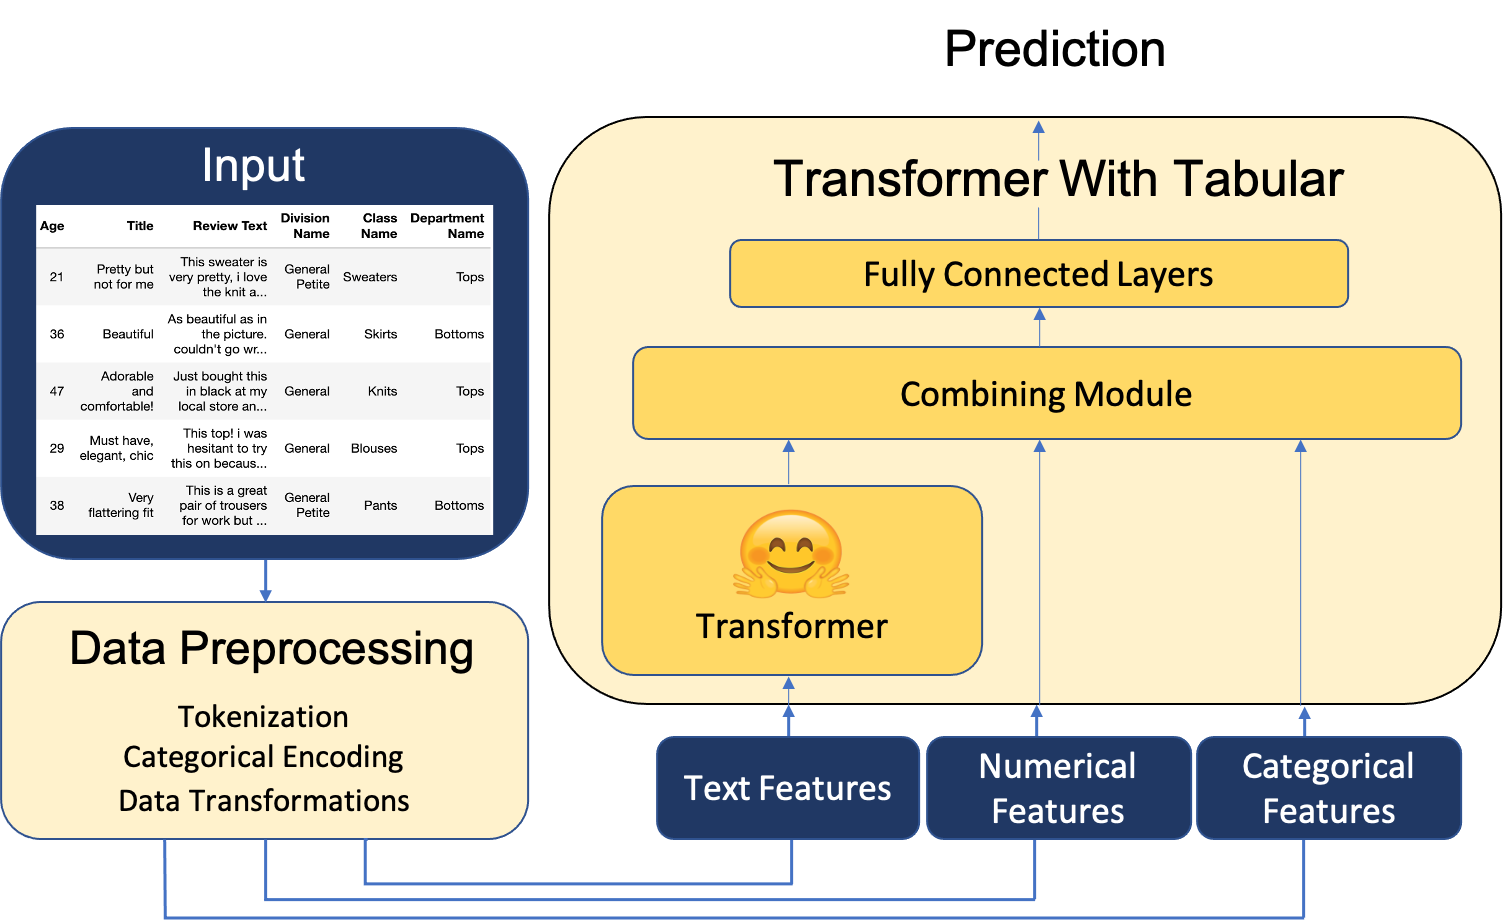
\includegraphics[width=0.45\textwidth]{images/multimodal_bert}
\caption{MultimodalBERT architecture}
\label{fig:multimodal_bert_architecture}
\end{figure}
\newline
\newline
\textbf{Model Architecture}
\newline
An overview of the MultimodalBERT architecture is given in Figure \ref{fig:multimodal_bert_architecture}. We have performed various experiments in which we performed a gated summation of the transformer outputs as well as the numerical and categorical features before final classifier layer. unfortunately we have not been able to achieve satisfactory performance on the task and have therefore discontinued the approach.

\subsection{BERTweet}


\begin{table}
\centering
\setlength\tabcolsep{2pt}
\begin{tabular}{lccc}
\hline 
\textbf{Model / Features} & Precision & Recall & F1 Score \\ \hline
SVM & 1 & 1 & 1 \\
BERT-Base & 1 & 1 & 1 \\
BERT-Base + MLP  & 1 pt & 1 & 1 \\
\hline
\end{tabular}
\label{tbl:evaluation_scores} 
\caption{Evaluation scores }
\end{table}

\subsection{Results}

\section{Task 2 - Rumour Analysis}

Perform some analyses to understand the nature COVID-19 rumours and how they differ to their non- rumour counterparts...

\section{Conclusion}


\bibliographystyle{acl_natbib}
\bibliography{acl2021}

%\appendix



\end{document}
